\documentclass{article}
\usepackage{tikz}
\usepackage{geometry}
\usepackage[dvipsnames]{xcolor}
\pagestyle{empty}
\usepackage{luatexja}
\renewcommand{\kanjifamilydefault}{\gtdefault}
\renewcommand{\familydefault}{\sfdefault}
\newcommand{\docpaperwidth}{12.8cm}
\newcommand{\docpaperheight}{9.6cm}
\geometry{
  papersize={\docpaperwidth,\docpaperheight},
  margin=0cm,
  ignoreall=true
}
\usetikzlibrary{backgrounds}
\usetikzlibrary{calc}

\newcommand{\strsizex}{9cm}
\newcommand{\strsizey}{3cm}


\newcommand{\insetx}{0.05cm}
\newcommand{\insety}{0.05cm}
\newcommand{\mbrsize}{0.2cm}
\newcommand{\uefisize}{0.5cm}

\newcommand{\mbrxs}{\insetx}
\newcommand{\mbrxe}{\mbrxs + \mbrsize}
\newcommand{\uefixs}{\mbrxe + \insetx}
\newcommand{\uefixe}{\uefixs + \uefisize}
\newcommand{\linuxxs}{\uefixe + \insetx}
\newcommand{\linuxxe}{\strsizex - \insetx}

\newcommand{\mbrys}{\insety}
\newcommand{\mbrye}{\strsizey - \insety}
\newcommand{\uefiys}{\insety}
\newcommand{\uefiye}{\strsizey - \insety}
\newcommand{\linuxys}{\insety}
\newcommand{\linuxye}{\strsizey - \insety}

\newcommand{\mbrnd}{($0.5*(\mbrxs + \mbrxe, \mbrys + \mbrye)$)}

\newcommand{\uefind}{($0.5*(\uefixs + \uefixe, \uefiys + \uefiye)$)}

\newcommand{\linuxnd}{($0.5*(\linuxxs + \linuxxe, \linuxys + \linuxye) $)}

% not used region for mbr backword compatible
\newcommand{\darkmbr}{
  \pgfpathrectanglecorners{\pgfpoint{\mbrxs}{\mbrys}}
    {\pgfpoint{\mbrxe}{\mbrye}}
}

% uifi partion
\newcommand{\uefipart}{
  \pgfpathrectanglecorners{\pgfpoint{\uefixs}{\uefiys}}
    {\pgfpoint{\uefixe}{\uefiye}}
}

% linux system partion
\newcommand{\linuxpart}{
  \pgfpathrectanglecorners{\pgfpoint{\linuxxs}{\linuxys}}
    {\pgfpoint{\linuxxe}{\linuxye}}
}

% entire storage
\newcommand{\entirestr}{
  \pgfpathrectanglecorners{\pgfpoint{0cm}{0cm}}
    {\pgfpoint{\strsizex}{\strsizey}}
}
  
\begin{document}
  \center
  % storage layout
  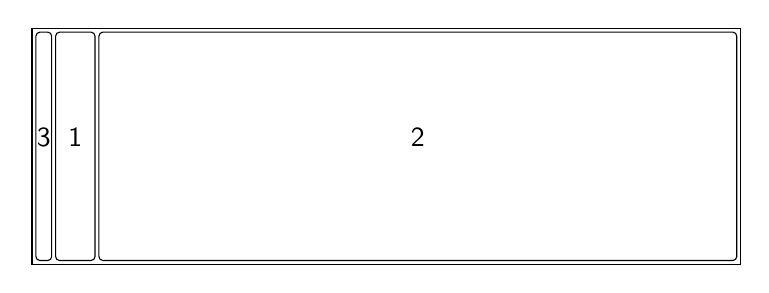
\begin{tikzpicture}[anchor=base]
    \node at \mbrnd {3};
    \node at \uefind {1};
    \node at \linuxnd {2};

    {
      \pgfsetcornersarced{\pgfpoint{0.05cm}{0.05cm}}
      % mbr part
      \darkmbr
      \pgfusepath{stroke}
      % uefi part
      \uefipart
      \pgfusepath{stroke}
      % linux part
      \linuxpart
      \pgfusepath{stroke}
    }

    \begin{scope}[on background layer]
      % entire ssd
      \entirestr
      \pgfusepath{stroke}
    \end{scope}
  \end{tikzpicture}
  \newpage
  % storage layout
  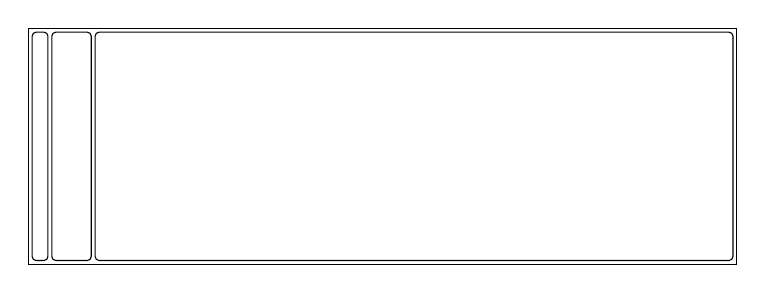
\begin{tikzpicture}[anchor=base,font=\tiny]
    {
      \pgfsetcornersarced{\pgfpoint{0.05cm}{0.05cm}}
      % mbr part
      \darkmbr
      \pgfusepath{stroke}
      % uefi part
      \uefipart
      \pgfusepath{stroke}
      % linux part
      \linuxpart
      \pgfusepath{stroke}
    }
    \begin{scope}[on background layer]
      % entire ssd
      \entirestr
      \pgfusepath{stroke}
    \end{scope}
  \end{tikzpicture}


\end{document} 
% vi: se ts=2 sw=2 et:
